%!TeX root=../carlo_master.tex
\chapter{Approaches to partition optimization}\label{sec:partition_optimization}

A line of work going back to \citet{obrien2008costsensitive} replaces the fixed analytical baseline with a learnable decision rule that minimizes empirical risk on a validation set, rather than relying on the theoretical partition derived from a potentially miscalibrated estimator. This chapter compares five parameterizations of that learnable rule: parallel shift on the cost matrix, linear scaling, probability-ratio thresholding, the multidimensional-thresholding view of \citet{legnaro2025multiclass}, and a priority-based sequential cascade. The first four induce convex-polytope partitions and are compared by which boundary normals each can express; they cluster into a hierarchy. Its top tier, $\mathcal{H}_{Full}$ (Section~\ref{sec:partition_matrix_framework}, Eq.~\ref{eq:hfull_def}), is the class of decision rules $\delta_{\mathbf{A}}(\mathbf{p}) = \underset{i \in \mathcal{Y}}{\mathrm{argmin}} \, \mathbf{a}_i^\top \mathbf{p}$ induced by an unconstrained learnable partition matrix $\mathbf{A} \in \mathbb{R}^{K \times K}$; its middle tier, $\mathcal{H}_{PS}$ (Eq.~\ref{eq:hps_def}), is the parallel-shift subclass that fixes the boundary normals at the cost-matrix differences but cannot rotate them. We collectively refer to the three classes $\mathcal{H}_{PS}$, $\mathcal{H}_{Sc}$, $\mathcal{H}_{Full}$, all parameterized through the partition matrix $\mathbf{A}$ of Section~\ref{sec:partition_matrix_framework}, as the \emph{matrix-parameterized methods}, and to the $K{-}1$-parameter subset $\mathcal{H}_{PS} \cup \mathcal{H}_{Sc}$, in which a single $K$-vector translates or rescales the cost-matrix columns, as the \emph{vector-tuned methods}. Their sample complexity is analysed together in Chapter~\ref{sec:voronoi_tessellation}. The sequential cascade sits outside this hierarchy: its decision regions are non-convex and order-dependent, and we include it as a heuristic contrast to the polytope methods.

\section{The partition matrix framework}\label{sec:partition_matrix_framework}

\citet{obrien2008costsensitive} formalized the problem of learning the decision rule from validation data as \textit{partition learning}: decouple the \textit{evaluation cost matrix} $\mathbf{C}$, which defines the ground-truth penalty, from the \textit{decision partition matrix} $\mathbf{A}$, which parameterizes the decision boundary.

Let $\mathbf{A} \in \mathbb{R}^{K \times K}$ be a learnable parameter matrix. The decision rule is defined as minimizing the ``apparent'' risk parameterized by $\mathbf{A}$,
\begin{equation}\label{eq:obrien_rule}
    \delta_{\mathbf{A}}(\mathbf{p}) = \underset{i \in \mathcal{Y}}{\mathrm{argmin}} \sum_{j=0}^{K-1} A_{ji} p_j = \underset{i \in \mathcal{Y}}{\mathrm{argmin}} \,\, \mathbf{a}_i^\top \mathbf{p},
\end{equation}
where $\mathbf{a}_i$ denotes the $i$-th column of $\mathbf{A}$ (the apparent costs of predicting class $i$ across all possible truth labels).
The optimization objective is to find the matrix $\mathbf{A}^*$ that minimizes the \textit{true} empirical risk, evaluated using $\mathbf{C}$ on the plug-in classifier $\delta_{\mathbf{A}} \circ \hat{\mathbf{p}}$, over the validation set $\mathcal{V}$,
\begin{equation}
    \mathbf{A}^* = \underset{\mathbf{A} \in \mathbb{R}^{K \times K}}{\mathrm{argmin}} \sum_{(x, y) \in \mathcal{V}} C_{y, \,\delta_{\mathbf{A}}(\hat{\mathbf{p}}(x))}.
\end{equation}
Choosing $\mathbf{A}^*$ by minimizing this empirical risk over $\mathcal{V}$ is the multiclass instance of the decision-stage learning problem (Section~\ref{sec:decision_learning}): empirical risk minimization over $\mathcal{H}_{dec}$, here parameterized by the partition matrix $\mathbf{A}$.
Learning all $K^2$ entries of $\mathbf{A}$ is prone to overfitting, which is why \citet{obrien2008costsensitive} proposed structural constraints on $\mathbf{A}$ corresponding to specific geometric transformations of the boundaries.

The admissibility and element-wise reasonableness conditions (Definitions~\ref{def:admissibility} and~\ref{def:elementwise}) constrain only the evaluation matrix $\mathbf{C}$. We place no such restriction on the decision matrix $\mathbf{A}$: the unconstrained partition class is
\begin{equation}\label{eq:hfull_def}
    \mathcal{H}_{Full} = \left\{ \delta(\mathbf{p}) = \underset{k \in \mathcal{Y}}{\mathrm{argmin}} \,\, \mathbf{a}_k^\top \mathbf{p} \mid \mathbf{A} \in \mathbb{R}^{K \times K} \right\},
\end{equation}
with $\mathbf{a}_k$ ranging over all of $\mathbb{R}^{K}$.

\section{Geometric regularization strategies}

The four constraints below sit on a spectrum of how aggressively they reduce $\mathcal{H}_{Full}$. All can be fit by empirical optimization on a validation set, so the learning objective need not be tied to a specified cost matrix: the same search can target cost-sensitive risk, macro $F_1$, macro G-Mean, or any other task utility. What distinguishes the methods below is not the optimization criterion but the geometry of the partitions they can express.

The first two (parallel shift and linear scaling) come from \citet{obrien2008costsensitive}; the third is the per-class probability rescaling of \citet{lachiche2003improving}, recast here in cost-agnostic form; the fourth, due to \citet{legnaro2025multiclass}, parameterizes the decision rule directly on the simplex and, as we show below, is mathematically equivalent to the parallel shift under $0/1$ loss.

\subsection{Parallel shift parameterization}\label{sec:parallel_shifts}

The strongest strategy identified by \citet{obrien2008costsensitive} constrains $\mathbf{A}$ to be a column-wise translation of $\mathbf{C}$, one bias per predicted class. Introducing a learnable bias vector $\boldsymbol{\alpha} \in \mathbb{R}^K$,
\begin{equation}
    A_{ij} = C_{ij} + \alpha_j.
\end{equation}
This formulation has $K-1$ degrees of freedom (since shifting all $\alpha_j$ by a constant does not change the argmin).

\begin{proposition}[Parallel boundary invariance]\label{prop:parallel_invariance}
    Let $\mathcal{B}_{ij}(\mathbf{C})$ be the theoretical decision boundary between class $i$ and $j$ induced by $\mathbf{C}$. The boundary $\mathcal{B}_{ij}(\mathbf{A})$ induced by the parallel shift parameterization is parallel to $\mathcal{B}_{ij}(\mathbf{C})$.
\end{proposition}

\begin{proof}
    The boundary between class $i$ and $j$ is the locus of points where the apparent risks are equal,
    \begin{align}
        \sum_{k=0}^{K-1} (C_{ki} + \alpha_i) p_k &= \sum_{k=0}^{K-1} (C_{kj} + \alpha_j) p_k \\
        \mathbf{c}_i^\top \mathbf{p} + \alpha_i \underbrace{\sum_{k=0}^{K-1} p_k}_{1} &= \mathbf{c}_j^\top \mathbf{p} + \alpha_j \underbrace{\sum_{k=0}^{K-1} p_k}_{1} \\
        (\mathbf{c}_i - \mathbf{c}_j)^\top \mathbf{p} + (\alpha_i - \alpha_j) &= 0.
    \end{align}
    The normal vector of this hyperplane remains $\mathbf{n}_{ij} = \mathbf{c}_i - \mathbf{c}_j$, identical to the theoretical boundary. The term $(\alpha_i - \alpha_j)$ acts as a scalar offset, translating the hyperplane along the normal vector.
\end{proof}

The parallel-shift constraint corrects monotonic calibration bias (global over- or undersmoothing in the sense of Section~\ref{sec:analytical_fragility}) without changing the cost-aware orientation of any boundary. When $\hat{\mathbf{p}}$ systematically underestimates a minority class $i$, the optimizer can lower $\alpha_i$ relative to the other classes to enlarge $\mathcal{P}_i^{\boldsymbol{\alpha}}$, leaving the relative trade-off between the remaining classes unchanged. Figure~\ref{fig:obrien_parallel_shifts} illustrates this on an asymmetric cost matrix: a lowered bias entry enlarges its region by translating the bordering boundaries while keeping every boundary normal fixed.

\begin{figure}[H]
    \centering
    \resizebox{\textwidth}{!}{\documentclass[tikz, border=10pt]{standalone}
\usepackage{tikz}
\usepackage{amsmath}
\usetikzlibrary{shapes, calc, backgrounds, arrows.meta}

\begin{document}
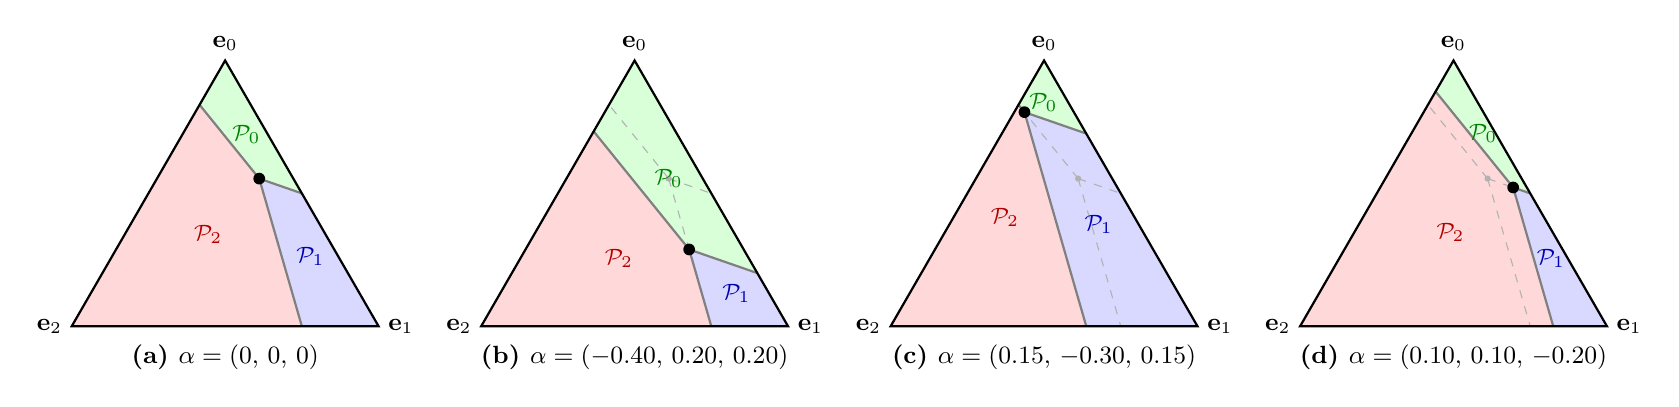
\begin{tikzpicture}[font=\sffamily]

    \begin{scope}[xshift=0.0cm, scale=0.45]
    \coordinate (Top) at (0.000, 5.000);
    \coordinate (Right) at (4.330, -2.500);
    \coordinate (Left) at (-4.330, -2.500);

    \coordinate (Int) at (0.962, 1.667);

    \fill[green!15] (0.000, 5.000) -- (2.165, 1.250) -- (0.962, 1.667) -- (-0.722, 3.750) -- cycle;
    \fill[blue!15] (4.330, -2.500) -- (2.165, -2.500) -- (0.962, 1.667) -- (2.165, 1.250) -- cycle;
    \fill[red!15] (-4.330, -2.500) -- (-0.722, 3.750) -- (0.962, 1.667) -- (2.165, -2.500) -- cycle;

    \draw[thick, black!50] (Int) -- (2.165, 1.250);
    \draw[thick, black!50] (Int) -- (-0.722, 3.750);
    \draw[thick, black!50] (Int) -- (2.165, -2.500);

    \draw[thick] (Top) -- (Right) -- (Left) -- cycle;

    \node[circle, fill=black, inner sep=1.5pt] at (Int) {};

    \node[green!50!black, font=\footnotesize\bfseries] at (0.601, 2.917) {$\mathcal{P}_0$};
    \node[blue!70!black, font=\footnotesize\bfseries] at (2.406, -0.521) {$\mathcal{P}_1$};
    \node[red!70!black, font=\footnotesize\bfseries] at (-0.481, 0.104) {$\mathcal{P}_2$};

    \node[above, font=\small] at (Top) {$\mathbf{e}_0$};
    \node[right, font=\small] at (Right) {$\mathbf{e}_1$};
    \node[left, font=\small] at (Left) {$\mathbf{e}_2$};
    \node[font=\small\bfseries, anchor=north, align=center] at (0, -2.750) {(a) $\boldsymbol{\alpha} = (0,\,0,\,0)$};
    \end{scope}

    \begin{scope}[xshift=5.2cm, scale=0.45]
    \coordinate (Top) at (0.000, 5.000);
    \coordinate (Right) at (4.330, -2.500);
    \coordinate (Left) at (-4.330, -2.500);

    \coordinate (Int) at (1.540, -0.333);

    \fill[green!15] (0.000, 5.000) -- (3.464, -1.000) -- (1.540, -0.333) -- (-1.155, 3.000) -- cycle;
    \fill[blue!15] (4.330, -2.500) -- (2.165, -2.500) -- (1.540, -0.333) -- (3.464, -1.000) -- cycle;
    \fill[red!15] (-4.330, -2.500) -- (-1.155, 3.000) -- (1.540, -0.333) -- (2.165, -2.500) -- cycle;

    \coordinate (OvInt) at (0.962, 1.667);
    \draw[dashed, gray!60, thin] (OvInt) -- (2.165, 1.250);
    \draw[dashed, gray!60, thin] (OvInt) -- (-0.722, 3.750);
    \draw[dashed, gray!60, thin] (OvInt) -- (2.165, -2.500);
    \node[circle, fill=gray!60, inner sep=0.8pt] at (OvInt) {};

    \draw[thick, black!50] (Int) -- (3.464, -1.000);
    \draw[thick, black!50] (Int) -- (-1.155, 3.000);
    \draw[thick, black!50] (Int) -- (2.165, -2.500);

    \draw[thick] (Top) -- (Right) -- (Left) -- cycle;

    \node[circle, fill=black, inner sep=1.5pt] at (Int) {};

    \node[green!50!black, font=\footnotesize\bfseries] at (0.962, 1.667) {$\mathcal{P}_0$};
    \node[blue!70!black, font=\footnotesize\bfseries] at (2.875, -1.583) {$\mathcal{P}_1$};
    \node[red!70!black, font=\footnotesize\bfseries] at (-0.445, -0.583) {$\mathcal{P}_2$};

    \node[above, font=\small] at (Top) {$\mathbf{e}_0$};
    \node[right, font=\small] at (Right) {$\mathbf{e}_1$};
    \node[left, font=\small] at (Left) {$\mathbf{e}_2$};
    \node[font=\small\bfseries, anchor=north, align=center] at (0, -2.750) {(b) $\boldsymbol{\alpha} = (-0.40,\,0.20,\,0.20)$};
    \end{scope}

    \begin{scope}[xshift=10.4cm, scale=0.45]
    \coordinate (Top) at (0.000, 5.000);
    \coordinate (Right) at (4.330, -2.500);
    \coordinate (Left) at (-4.330, -2.500);

    \coordinate (Int) at (-0.553, 3.542);

    \fill[green!15] (0.000, 5.000) -- (1.191, 2.938) -- (-0.553, 3.542) -- (-0.722, 3.750) -- cycle;
    \fill[blue!15] (4.330, -2.500) -- (1.191, -2.500) -- (-0.553, 3.542) -- (1.191, 2.938) -- cycle;
    \fill[red!15] (-4.330, -2.500) -- (-0.722, 3.750) -- (-0.553, 3.542) -- (1.191, -2.500) -- cycle;

    \coordinate (OvInt) at (0.962, 1.667);
    \draw[dashed, gray!60, thin] (OvInt) -- (2.165, 1.250);
    \draw[dashed, gray!60, thin] (OvInt) -- (-0.722, 3.750);
    \draw[dashed, gray!60, thin] (OvInt) -- (2.165, -2.500);
    \node[circle, fill=gray!60, inner sep=0.8pt] at (OvInt) {};

    \draw[thick, black!50] (Int) -- (1.191, 2.938);
    \draw[thick, black!50] (Int) -- (-0.722, 3.750);
    \draw[thick, black!50] (Int) -- (1.191, -2.500);

    \draw[thick] (Top) -- (Right) -- (Left) -- cycle;

    \node[circle, fill=black, inner sep=1.5pt] at (Int) {};

    \node[green!50!black, font=\footnotesize\bfseries] at (-0.021, 3.807) {$\mathcal{P}_0$};
    \node[blue!70!black, font=\footnotesize\bfseries] at (1.540, 0.370) {$\mathcal{P}_1$};
    \node[red!70!black, font=\footnotesize\bfseries] at (-1.104, 0.573) {$\mathcal{P}_2$};

    \node[above, font=\small] at (Top) {$\mathbf{e}_0$};
    \node[right, font=\small] at (Right) {$\mathbf{e}_1$};
    \node[left, font=\small] at (Left) {$\mathbf{e}_2$};
    \node[font=\small\bfseries, anchor=north, align=center] at (0, -2.750) {(c) $\boldsymbol{\alpha} = (0.15,\,-0.30,\,0.15)$};
    \end{scope}

    \begin{scope}[xshift=15.600000000000001cm, scale=0.45]
    \coordinate (Top) at (0.000, 5.000);
    \coordinate (Right) at (4.330, -2.500);
    \coordinate (Left) at (-4.330, -2.500);

    \coordinate (Int) at (1.684, 1.417);

    \fill[green!15] (0.000, 5.000) -- (2.165, 1.250) -- (1.684, 1.417) -- (-0.505, 4.125) -- cycle;
    \fill[blue!15] (4.330, -2.500) -- (2.815, -2.500) -- (1.684, 1.417) -- (2.165, 1.250) -- cycle;
    \fill[red!15] (-4.330, -2.500) -- (-0.505, 4.125) -- (1.684, 1.417) -- (2.815, -2.500) -- cycle;

    \coordinate (OvInt) at (0.962, 1.667);
    \draw[dashed, gray!60, thin] (OvInt) -- (2.165, 1.250);
    \draw[dashed, gray!60, thin] (OvInt) -- (-0.722, 3.750);
    \draw[dashed, gray!60, thin] (OvInt) -- (2.165, -2.500);
    \node[circle, fill=gray!60, inner sep=0.8pt] at (OvInt) {};

    \draw[thick, black!50] (Int) -- (2.165, 1.250);
    \draw[thick, black!50] (Int) -- (-0.505, 4.125);
    \draw[thick, black!50] (Int) -- (2.815, -2.500);

    \draw[thick] (Top) -- (Right) -- (Left) -- cycle;

    \node[circle, fill=black, inner sep=1.5pt] at (Int) {};

    \node[green!50!black, font=\footnotesize\bfseries] at (0.836, 2.948) {$\mathcal{P}_0$};
    \node[blue!70!black, font=\footnotesize\bfseries] at (2.748, -0.583) {$\mathcal{P}_1$};
    \node[red!70!black, font=\footnotesize\bfseries] at (-0.084, 0.135) {$\mathcal{P}_2$};

    \node[above, font=\small] at (Top) {$\mathbf{e}_0$};
    \node[right, font=\small] at (Right) {$\mathbf{e}_1$};
    \node[left, font=\small] at (Left) {$\mathbf{e}_2$};
    \node[font=\small\bfseries, anchor=north, align=center] at (0, -2.750) {(d) $\boldsymbol{\alpha} = (0.10,\,0.10,\,-0.20)$};
    \end{scope}

\end{tikzpicture}
\end{document}
}
    \caption{O'Brien's parallel-shift regularization on the asymmetric cost matrix $\mathbf{C}$ with $C_{20}=5$, $C_{21}=3$ (same as panel~(b) of Figure~\ref{fig:simplex_cost_partition}). Panel~(a) shows the baseline $\mathbf{A}=\mathbf{C}$. Panels~(b)--(d) show $\mathbf{A}=\mathbf{C}+\mathbf{1}\boldsymbol{\alpha}^\top$ for three choices of the bias vector $\boldsymbol{\alpha}$, with dashed gray segments reproducing panel~(a)'s boundaries for reference. In each panel one entry of $\boldsymbol{\alpha}$ is set below the other two equal entries. Since $\mathcal{B}_{ij}$ depends only on $\alpha_i-\alpha_j$, the two boundaries bordering the favored class $i$ translate parallel to themselves and enlarge $\mathcal{P}_i^{\boldsymbol{\alpha}}$, while the boundary between the two equal-bias classes stays fixed (Proposition~\ref{prop:parallel_invariance}).}\label{fig:obrien_parallel_shifts}
\end{figure}

\subsection{Linear class scaling}\label{sec:linear_scaling}

An alternative parameterization scales each truth class by a learnable weight (a row-wise scaling under our convention; this corresponds to the column-wise scaling of \citet{obrien2008costsensitive}, who index $\mathbf{C}$ with the transposed convention). Let $\boldsymbol{\beta} \in \mathbb{R}^K_{\ge 0}$ be a vector of scaling factors, such that
\begin{equation}
    A_{ij} = C_{ij} \beta_i.
\end{equation}
This transformation is equivalent to modifying the estimated probabilities themselves, effectively replacing $\hat{p}_j(x)$ with a reweighted $\hat{p}'_j(x) \propto \beta_j \hat{p}_j(x)$.

\begin{proposition}[Boundary rotation under linear scaling]\label{prop:column_rotation}
    Unlike parallel shifts, linear scaling rotates the decision boundaries. Specifically, the boundary between classes $i$ and $j$ under linear scaling has normal vector $\mathbf{n}_{ij}^{(\boldsymbol{\beta})} = [(C_{0i} - C_{0j})\beta_0, \ldots, (C_{K-1,i} - C_{K-1,j})\beta_{K-1}]^\top$, which is in general not proportional to the unscaled normal $\mathbf{c}_i - \mathbf{c}_j$.
\end{proposition}

\begin{proof}
Under linear scaling, the decision boundary between classes $i$ and $j$ is the locus where their modified risks are equal,
\begin{equation}
    \sum_{k=0}^{K-1} C_{ki} \beta_k p_k = \sum_{k=0}^{K-1} C_{kj} \beta_k p_k.
\end{equation}
Rearranging yields $\sum_{k=0}^{K-1} (C_{ki} - C_{kj}) \beta_k p_k = 0$, which defines a hyperplane with normal vector
\begin{equation}
    \mathbf{n}_{ij}^{(\boldsymbol{\beta})} = \left[(C_{0i} - C_{0j})\beta_0, \; \ldots, \; (C_{K-1,i} - C_{K-1,j})\beta_{K-1}\right]^\top.
\end{equation}
In contrast, the unscaled normal is $\mathbf{n}_{ij} = \mathbf{c}_i - \mathbf{c}_j$, with components $(C_{ki} - C_{kj})$. The scaled normal $\mathbf{n}_{ij}^{(\boldsymbol{\beta})}$ is obtained by component-wise multiplication with $\boldsymbol{\beta}$, so $\mathbf{n}_{ij}^{(\boldsymbol{\beta})} = \boldsymbol{\beta} \odot \mathbf{n}_{ij}$, where $\odot$ denotes the Hadamard (element-wise) product. If $\boldsymbol{\beta}$ is not proportional to $\mathbf{1}$ and $\mathbf{n}_{ij}$ has at least two nonzero components with distinct $\beta$ values, then $\mathbf{n}_{ij}^{(\boldsymbol{\beta})} \not\propto \mathbf{n}_{ij}$, confirming that the boundary has rotated.
\end{proof}

Linear scaling is closely related to the per-class probability weighting of \citet{lachiche2003improving}, who learn one multiplicative weight per class for the estimated probabilities by greedy hill-climbing. Geometrically, this is the same kind of operation described above: it changes the boundary normals by reweighting the coordinates of the probability simplex.

Figure~\ref{fig:obrien_vs_column_scaling} contrasts the linear scaling with the parallel-shift parameterizations on a shared asymmetric cost matrix.

\begin{figure}[H]
    \centering
    \resizebox{\textwidth}{!}{\documentclass[tikz, border=10pt]{standalone}
\usepackage{tikz}
\usepackage{amsmath}
\usetikzlibrary{shapes, calc, backgrounds, arrows.meta}

\begin{document}
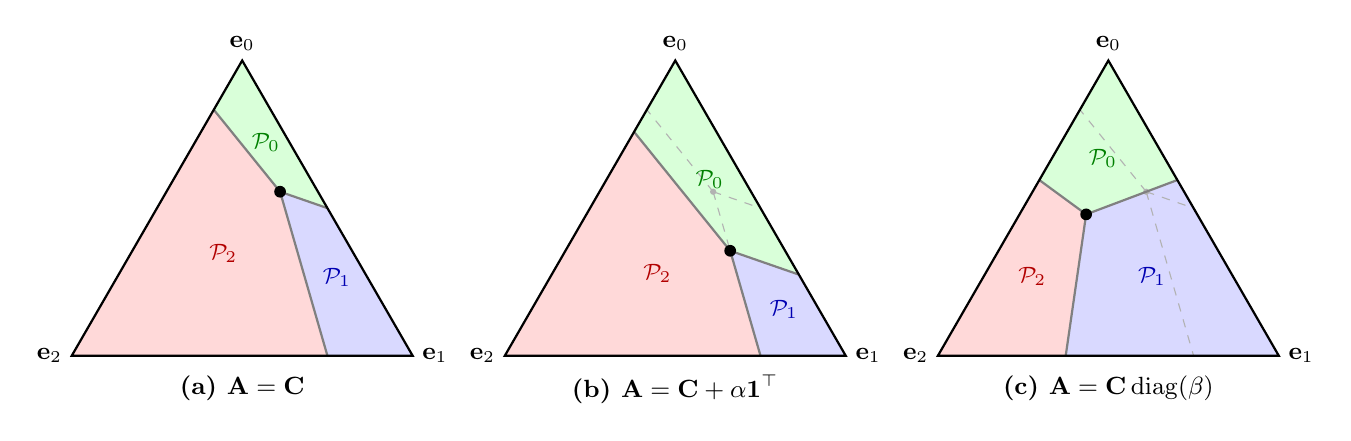
\begin{tikzpicture}[font=\sffamily]

    \begin{scope}[xshift=0.0cm, scale=0.5]
    \coordinate (Top) at (0.000, 5.000);
    \coordinate (Right) at (4.330, -2.500);
    \coordinate (Left) at (-4.330, -2.500);

    \coordinate (Int) at (0.962, 1.667);

    \fill[green!15] (0.000, 5.000) -- (2.165, 1.250) -- (0.962, 1.667) -- (-0.722, 3.750) -- cycle;
    \fill[blue!15] (4.330, -2.500) -- (2.165, -2.500) -- (0.962, 1.667) -- (2.165, 1.250) -- cycle;
    \fill[red!15] (-4.330, -2.500) -- (-0.722, 3.750) -- (0.962, 1.667) -- (2.165, -2.500) -- cycle;

    \draw[thick, black!50] (Int) -- (2.165, 1.250);
    \draw[thick, black!50] (Int) -- (-0.722, 3.750);
    \draw[thick, black!50] (Int) -- (2.165, -2.500);

    \draw[thick] (Top) -- (Right) -- (Left) -- cycle;

    \node[circle, fill=black, inner sep=1.5pt] at (Int) {};

    \node[green!50!black, font=\footnotesize\bfseries] at (0.601, 2.917) {$\mathcal{P}_0$};
    \node[blue!70!black, font=\footnotesize\bfseries] at (2.406, -0.521) {$\mathcal{P}_1$};
    \node[red!70!black, font=\footnotesize\bfseries] at (-0.481, 0.104) {$\mathcal{P}_2$};

    \node[above, font=\small] at (Top) {$\mathbf{e}_0$};
    \node[right, font=\small] at (Right) {$\mathbf{e}_1$};
    \node[left, font=\small] at (Left) {$\mathbf{e}_2$};
    \node[font=\small\bfseries, anchor=north, align=center] at (0, -2.750) {(a) $\mathbf{A} = \mathbf{C}$};
    \end{scope}

    \begin{scope}[xshift=5.5cm, scale=0.5]
    \coordinate (Top) at (0.000, 5.000);
    \coordinate (Right) at (4.330, -2.500);
    \coordinate (Left) at (-4.330, -2.500);

    \coordinate (Int) at (1.395, 0.167);

    \fill[green!15] (0.000, 5.000) -- (3.139, -0.438) -- (1.395, 0.167) -- (-1.046, 3.188) -- cycle;
    \fill[blue!15] (4.330, -2.500) -- (2.165, -2.500) -- (1.395, 0.167) -- (3.139, -0.438) -- cycle;
    \fill[red!15] (-4.330, -2.500) -- (-1.046, 3.188) -- (1.395, 0.167) -- (2.165, -2.500) -- cycle;

    \coordinate (OvInt) at (0.962, 1.667);
    \draw[dashed, gray!60, thin] (OvInt) -- (2.165, 1.250);
    \draw[dashed, gray!60, thin] (OvInt) -- (-0.722, 3.750);
    \draw[dashed, gray!60, thin] (OvInt) -- (2.165, -2.500);
    \node[circle, fill=gray!60, inner sep=0.8pt] at (OvInt) {};

    \draw[thick, black!50] (Int) -- (3.139, -0.438);
    \draw[thick, black!50] (Int) -- (-1.046, 3.188);
    \draw[thick, black!50] (Int) -- (2.165, -2.500);

    \draw[thick] (Top) -- (Right) -- (Left) -- cycle;

    \node[circle, fill=black, inner sep=1.5pt] at (Int) {};

    \node[green!50!black, font=\footnotesize\bfseries] at (0.872, 1.979) {$\mathcal{P}_0$};
    \node[blue!70!black, font=\footnotesize\bfseries] at (2.757, -1.318) {$\mathcal{P}_1$};
    \node[red!70!black, font=\footnotesize\bfseries] at (-0.454, -0.411) {$\mathcal{P}_2$};

    \node[above, font=\small] at (Top) {$\mathbf{e}_0$};
    \node[right, font=\small] at (Right) {$\mathbf{e}_1$};
    \node[left, font=\small] at (Left) {$\mathbf{e}_2$};
    \node[font=\small\bfseries, anchor=north, align=center] at (0, -2.750) {(b) $\mathbf{A} = \mathbf{C} + \boldsymbol{\alpha}\mathbf{1}^\top$};
    \end{scope}

    \begin{scope}[xshift=11.0cm, scale=0.5]
    \coordinate (Top) at (0.000, 5.000);
    \coordinate (Right) at (4.330, -2.500);
    \coordinate (Left) at (-4.330, -2.500);

    \coordinate (Int) at (-0.564, 1.092);

    \fill[green!15] (0.000, 5.000) -- (1.753, 1.964) -- (-0.564, 1.092) -- (-1.753, 1.964) -- cycle;
    \fill[blue!15] (4.330, -2.500) -- (-1.083, -2.500) -- (-0.564, 1.092) -- (1.753, 1.964) -- cycle;
    \fill[red!15] (-4.330, -2.500) -- (-1.753, 1.964) -- (-0.564, 1.092) -- (-1.083, -2.500) -- cycle;

    \coordinate (OvInt) at (0.962, 1.667);
    \draw[dashed, gray!60, thin] (OvInt) -- (2.165, 1.250);
    \draw[dashed, gray!60, thin] (OvInt) -- (-0.722, 3.750);
    \draw[dashed, gray!60, thin] (OvInt) -- (2.165, -2.500);
    \node[circle, fill=gray!60, inner sep=0.8pt] at (OvInt) {};

    \draw[thick, black!50] (Int) -- (1.753, 1.964);
    \draw[thick, black!50] (Int) -- (-1.753, 1.964);
    \draw[thick, black!50] (Int) -- (-1.083, -2.500);

    \draw[thick] (Top) -- (Right) -- (Left) -- cycle;

    \node[circle, fill=black, inner sep=1.5pt] at (Int) {};

    \node[green!50!black, font=\footnotesize\bfseries] at (-0.141, 2.505) {$\mathcal{P}_0$};
    \node[blue!70!black, font=\footnotesize\bfseries] at (1.109, -0.486) {$\mathcal{P}_1$};
    \node[red!70!black, font=\footnotesize\bfseries] at (-1.932, -0.486) {$\mathcal{P}_2$};

    \node[above, font=\small] at (Top) {$\mathbf{e}_0$};
    \node[right, font=\small] at (Right) {$\mathbf{e}_1$};
    \node[left, font=\small] at (Left) {$\mathbf{e}_2$};
    \node[font=\small\bfseries, anchor=north, align=center] at (0, -2.750) {(c) $\mathbf{A} = \mathbf{C}\,\mathrm{diag}(\boldsymbol{\beta})$};
    \end{scope}

\end{tikzpicture}
\end{document}
}
    \caption{Parallel shift versus linear scaling applied to the same asymmetric $\mathbf{C}$ as Figure~\ref{fig:obrien_parallel_shifts}. Panel~(a) is the baseline $\mathbf{A}=\mathbf{C}$. Panel~(b) adds a per-prediction-class bias $\boldsymbol{\alpha}=(-0.30,\,0.15,\,0.15)$: the boundaries translate but retain the normals $\mathbf{n}_{ij}=\mathbf{c}_i-\mathbf{c}_j$ (Proposition~\ref{prop:parallel_invariance}). Panel~(c) applies a linear scaling $\boldsymbol{\beta}=(3.4,\,5.0,\,1.0)$; the dashed baseline shows that the solid boundaries are \emph{rotated}, not merely shifted (Proposition~\ref{prop:column_rotation}). When the cost structure is known, the parallel-shift parameterization respects it by construction; linear scaling does not.}\label{fig:obrien_vs_column_scaling}
\end{figure}

\subsection{Probability ratio thresholding}\label{sec:prob_ratio_thresholding}

An alternative to linear scaling that avoids direct manipulation of the cost matrix is \textit{Probability Ratio Thresholding}, the per-class probability reweighting of \citet{lachiche2003improving}, stated here as a decision rule rather than a probability correction. Rather than modifying the risk computation, this method rescales the estimated probabilities directly,
\begin{equation}\label{eq:threshold_ratio}
    \delta_{\boldsymbol{\tau}}(\mathbf{p}) = \underset{k \in \mathcal{Y}}{\mathrm{argmax}} \; \frac{p_k}{\tau_k},
\end{equation}
where $\boldsymbol{\tau} \in \mathbb{R}_{>0}^K$ is a per-class threshold vector. To remove scale invariance, we fix $\tau_0 = 1$, yielding $K-1$ free parameters.

\begin{proposition}[Equivalence to linear scaling under 0/1 loss]\label{prop:ratio_equivalence}
    Under the 0/1 loss matrix ($C_{ij} = 1 - \delta_{ij}$), Probability Ratio Thresholding with parameter $\boldsymbol{\tau}$ is equivalent to linear scaling with $\beta_k = 1/\tau_k$.
\end{proposition}

\begin{proof}
    Under 0/1 loss, the risk of predicting class $i$ given $\mathbf{p}$ is $\mathcal{L}_i(\mathbf{p}) = \sum_{j \neq i} p_j = 1 - p_i$. The standard analytical rule is $\mathrm{argmin}_{k \in \mathcal{Y}}(1 - p_k) = \mathrm{argmax}_{k \in \mathcal{Y}}\, p_k$. Applying linear scaling with $\boldsymbol{\beta}$ gives $\mathrm{argmin}_{k \in \mathcal{Y}}\sum_{j \neq k} \beta_j p_j = \mathrm{argmin}_{k \in \mathcal{Y}}(\sum_j \beta_j p_j - \beta_k p_k)$. Since $\sum_j \beta_j p_j$ is independent of $k$, this reduces to $\mathrm{argmax}_{k \in \mathcal{Y}}\, \beta_k p_k$. Setting $\beta_k = 1/\tau_k$ yields $\mathrm{argmax}_{k \in \mathcal{Y}}\, p_k / \tau_k$, which is exactly Eq.~\ref{eq:threshold_ratio}.
\end{proof}

Under $0/1$ loss, linear scaling and probability-ratio thresholding thus parameterize the same hypothesis class, the column-scaling counterpart of $\mathcal{H}_{PS}$, which we denote
\begin{equation}\label{eq:hsc_def}
    \mathcal{H}_{Sc} = \left\{ \delta(\mathbf{p}) = \underset{i \in \mathcal{Y}}{\mathrm{argmin}} \sum_{k=0}^{K-1} C_{ki}\, \beta_k\, p_k \;\middle|\; \boldsymbol{\beta} \in \mathbb{R}_{>0}^K,\; \beta_0 = 1 \right\}.
\end{equation}
The gauge $\beta_0 = 1$ pins down the one-dimensional scaling invariance $\arg\min_k(c\, s_k) = \arg\min_k s_k$ for any $c > 0$, so $\mathcal{H}_{Sc}$ has $K-1$ free parameters, the same budget as $\mathcal{H}_{PS}$. Its boundary normals rotate with $\boldsymbol{\beta}$ (Proposition~\ref{prop:column_rotation}) rather than staying fixed at $\mathbf{c}_i - \mathbf{c}_j$, so $\mathcal{H}_{Sc}$ and $\mathcal{H}_{PS}$ are distinct restricted classes at the same complexity, not nested.

\subsection{Multidimensional thresholding}\label{sec:multidim_thresholding}

\citet{legnaro2025multiclass} reformulate the parallel-shift rule directly on the simplex, sidestepping the cost matrix entirely. Their decision rule selects the class with the largest threshold-shifted probability,
\begin{equation}
    \delta(\mathbf{p}) = \underset{k \in \mathcal{Y}}{\mathrm{argmax}} \,\, (p_k - \tau_k),
\end{equation}
parameterized by a threshold vector $\boldsymbol{\tau} \in \Delta^{K-1}$, with the corresponding decision regions
\begin{equation}
    \mathcal{P}_j^{\boldsymbol{\tau}} = \left\{ \mathbf{p} \in \Delta^{K-1} \mid p_j - p_k > \tau_j - \tau_k, \, \forall k \neq j \right\}.
\end{equation}
Unlike probability-ratio thresholding, which rescales the simplex coordinates and rotates the induced boundaries, multidimensional thresholding translates the argmax partition: the pairwise boundaries remain hyperplanes with normals $\mathbf{n}_{ij} = \mathbf{e}_i - \mathbf{e}_j$, but their common intersection is moved away from the barycenter (Figure~\ref{fig:marchetti_thresholding}).

\begin{proposition}[Equivalence to parallel-shift regularization]\label{prop:marchetti_equivalence}
    With the threshold vector allowed to range over $\mathbb{R}^K$, multidimensional thresholding is equivalent to the parallel-shift strategy applied to the $0/1$ loss matrix.
\end{proposition}

\begin{proof}
    Under the $0/1$ cost matrix ($C_{ij} = 1 - \delta_{ij}$), the parallel-shift rule of Section~\ref{sec:partition_optimization} reduces to
    \begin{equation}
        \underset{k \in \mathcal{Y}}{\mathrm{argmin}} \,\, (1 - p_k) + \alpha_k = \underset{k \in \mathcal{Y}}{\mathrm{argmax}} \,\, (p_k - \alpha_k).
    \end{equation}
    Setting $\alpha_k = \tau_k$ recovers the multidimensional-thresholding rule.
\end{proof}

The equivalence is exact only under $0/1$ loss; for asymmetric cost matrices the parallel-shift parameterization on $\mathbf{C}$ exploits cost-matrix structure that the simplex-side $\boldsymbol{\tau}$ does not see.

\begin{figure}[H]
    \centering
    \resizebox{\textwidth}{!}{\documentclass[tikz, border=10pt]{standalone}
\usepackage{tikz}
\usepackage{amsmath}
\usetikzlibrary{shapes, calc, backgrounds, arrows.meta}

\begin{document}
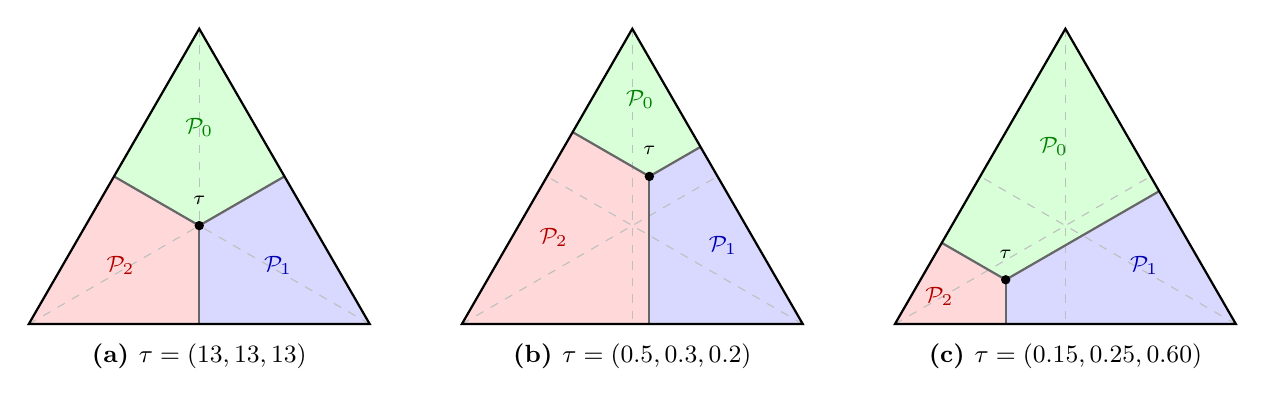
\begin{tikzpicture}[font=\sffamily]

    \begin{scope}[xshift=0.0cm, scale=0.5]
    \coordinate (Top) at (0.000, 5.000);
    \coordinate (Right) at (4.330, -2.500);
    \coordinate (Left) at (-4.330, -2.500);

    \coordinate (Int) at (0.000, 0.000);

    \fill[green!15] (0.000, 5.000) -- (2.165, 1.250) -- (0.000, 0.000) -- (-2.165, 1.250) -- cycle;
    \fill[blue!15] (4.330, -2.500) -- (0.000, -2.500) -- (0.000, 0.000) -- (2.165, 1.250) -- cycle;
    \fill[red!15] (-4.330, -2.500) -- (-2.165, 1.250) -- (0.000, 0.000) -- (0.000, -2.500) -- cycle;

    \draw[dashed, gray!50, thin] (Left) -- (2.165, 1.250);
    \draw[dashed, gray!50, thin] (Right) -- (-2.165, 1.250);
    \draw[dashed, gray!50, thin] (Top) -- (0.000, -2.500);

    \draw[thick, black!60] (Int) -- (2.165, 1.250);
    \draw[thick, black!60] (Int) -- (-2.165, 1.250);
    \draw[thick, black!60] (Int) -- (0.000, -2.500);

    \node[circle, fill=black, inner sep=1.2pt] at (Int) {};
    \node[font=\scriptsize, anchor=south] at (0.000, 0.300) {$\boldsymbol{\tau}$};

    \draw[thick] (Top) -- (Right) -- (Left) -- cycle;

    \node[green!50!black, font=\footnotesize\bfseries] at (0.000, 2.500) {$\mathcal{P}_0$};
    \node[blue!70!black, font=\footnotesize\bfseries] at (2.000, -1.000) {$\mathcal{P}_1$};
    \node[red!70!black, font=\footnotesize\bfseries] at (-2.000, -1.000) {$\mathcal{P}_2$};

    \node[font=\small\bfseries, anchor=north, align=center] at (0, -2.750) {(a) $\boldsymbol{\tau} = (\tfrac{1}{3},\tfrac{1}{3},\tfrac{1}{3})$};
    \end{scope}

    \begin{scope}[xshift=5.5cm, scale=0.5]
    \coordinate (Top) at (0.000, 5.000);
    \coordinate (Right) at (4.330, -2.500);
    \coordinate (Left) at (-4.330, -2.500);

    \coordinate (Int) at (0.433, 1.250);

    \fill[green!15] (0.000, 5.000) -- (1.732, 2.000) -- (0.433, 1.250) -- (-1.516, 2.375) -- cycle;
    \fill[blue!15] (4.330, -2.500) -- (0.433, -2.500) -- (0.433, 1.250) -- (1.732, 2.000) -- cycle;
    \fill[red!15] (-4.330, -2.500) -- (-1.516, 2.375) -- (0.433, 1.250) -- (0.433, -2.500) -- cycle;

    \draw[dashed, gray!50, thin] (Left) -- (2.165, 1.250);
    \draw[dashed, gray!50, thin] (Right) -- (-2.165, 1.250);
    \draw[dashed, gray!50, thin] (Top) -- (0.000, -2.500);

    \draw[thick, black!60] (Int) -- (1.732, 2.000);
    \draw[thick, black!60] (Int) -- (-1.516, 2.375);
    \draw[thick, black!60] (Int) -- (0.433, -2.500);

    \node[circle, fill=black, inner sep=1.2pt] at (Int) {};
    \node[font=\scriptsize, anchor=south] at (0.433, 1.550) {$\boldsymbol{\tau}$};

    \draw[thick] (Top) -- (Right) -- (Left) -- cycle;

    \node[green!50!black, font=\footnotesize\bfseries] at (0.200, 3.200) {$\mathcal{P}_0$};
    \node[blue!70!black, font=\footnotesize\bfseries] at (2.300, -0.500) {$\mathcal{P}_1$};
    \node[red!70!black, font=\footnotesize\bfseries] at (-2.000, -0.300) {$\mathcal{P}_2$};

    \node[font=\small\bfseries, anchor=north, align=center] at (0, -2.750) {(b) $\boldsymbol{\tau} = (0.5, 0.3, 0.2)$};
    \end{scope}

    \begin{scope}[xshift=11.0cm, scale=0.5]
    \coordinate (Top) at (0.000, 5.000);
    \coordinate (Right) at (4.330, -2.500);
    \coordinate (Left) at (-4.330, -2.500);

    \coordinate (Int) at (-1.516, -1.375);

    \fill[green!15] (0.000, 5.000) -- (2.382, 0.875) -- (-1.516, -1.375) -- (-3.139, -0.438) -- cycle;
    \fill[blue!15] (4.330, -2.500) -- (-1.516, -2.500) -- (-1.516, -1.375) -- (2.382, 0.875) -- cycle;
    \fill[red!15] (-4.330, -2.500) -- (-3.139, -0.438) -- (-1.516, -1.375) -- (-1.516, -2.500) -- cycle;

    \draw[dashed, gray!50, thin] (Left) -- (2.165, 1.250);
    \draw[dashed, gray!50, thin] (Right) -- (-2.165, 1.250);
    \draw[dashed, gray!50, thin] (Top) -- (0.000, -2.500);

    \draw[thick, black!60] (Int) -- (2.382, 0.875);
    \draw[thick, black!60] (Int) -- (-3.139, -0.438);
    \draw[thick, black!60] (Int) -- (-1.516, -2.500);

    \node[circle, fill=black, inner sep=1.2pt] at (Int) {};
    \node[font=\scriptsize, anchor=south] at (-1.516, -1.075) {$\boldsymbol{\tau}$};

    \draw[thick] (Top) -- (Right) -- (Left) -- cycle;

    \node[green!50!black, font=\footnotesize\bfseries] at (-0.300, 2.000) {$\mathcal{P}_0$};
    \node[blue!70!black, font=\footnotesize\bfseries] at (2.000, -1.000) {$\mathcal{P}_1$};
    \node[red!70!black, font=\footnotesize\bfseries] at (-3.200, -1.800) {$\mathcal{P}_2$};

    \node[font=\small\bfseries, anchor=north, align=center] at (0, -2.750) {(c) $\boldsymbol{\tau} = (0.15, 0.25, 0.60)$};
    \end{scope}

\end{tikzpicture}
\end{document}
}
    \caption{Effect of the threshold vector $\boldsymbol{\tau}$ on the multidimensional thresholding rule. The decision rule $\delta(\mathbf{p}) = \operatorname{argmax}_{k \in \mathcal{Y}} (p_k - \tau_k)$ produces boundaries parallel to the argmax medians (dashed gray), with the intersection point shifted from the barycenter $G$ to $\boldsymbol{\tau}$ (black dot). A larger $\tau_k$ penalizes class~$k$, shrinking $\mathcal{P}_k^{\boldsymbol{\tau}}$: \textbf{(a)}~equal thresholds recover the standard argmax partition; \textbf{(b)}~$\tau_0 = 0.5$ shrinks $\mathcal{P}_0^{\boldsymbol{\tau}}$; \textbf{(c)}~$\tau_2 = 0.60$ shrinks $\mathcal{P}_2^{\boldsymbol{\tau}}$, expanding $\mathcal{P}_0^{\boldsymbol{\tau}}$.}\label{fig:marchetti_thresholding}
\end{figure}

\citeauthor{obrien2008costsensitive}'s parallel shifts and \citeauthor{legnaro2025multiclass}'s multidimensional thresholding are thus the same restricted class when $\boldsymbol{\tau}$ ranges over $\mathbb{R}^K$, in which boundaries are parameterized by a single vector $\mathbf{v} \in \mathbb{R}^K$ (either the bias $\boldsymbol{\alpha}$ or the threshold $\boldsymbol{\tau}$),
\begin{equation}\label{eq:hps_def}
    \mathcal{H}_{PS} = \left\{ \delta(\mathbf{p}) = \underset{k \in \mathcal{Y}}{\mathrm{argmin}} \,\, (\mathbf{c}_k^\top \mathbf{p} + v_k) \mid \mathbf{v} \in \mathbb{R}^{K}, \sum v_k = 0 \right\}.
\end{equation}
The mean-zero gauge $\sum_k v_k = 0$ pins down the one-dimensional translation invariance $\arg\min_{k \in \mathcal{Y}}(s_k + c) = \arg\min_{k \in \mathcal{Y}} s_k$ for any scalar $c$. The accompanying code adopts the equivalent first-coordinate gauge $v_0 = 0$ instead and searches the remaining $K-1$ coordinates; the two parameterizations yield identical decision rules but the recorded bias vectors differ by the additive constant $-\overline{v}$. Linear scaling (Section~\ref{sec:linear_scaling}) and probability-ratio thresholding (Section~\ref{sec:prob_ratio_thresholding}) form the column-scaling sibling $\mathcal{H}_{Sc}$ (Eq.~\ref{eq:hsc_def}) at the same $K-1$ parameter budget but outside $\mathcal{H}_{PS}$: their boundary normals are rotated by the per-class scaling (Proposition~\ref{prop:column_rotation}) rather than fixed at $\mathbf{c}_i - \mathbf{c}_j$.

\subsection{Priority-based sequential selection}\label{sec:sequential_selection}

An alternative heuristic, motivated by class-imbalanced settings, applies per-class binary thresholds in a sequential cascade that processes classes in an explicit priority order. This construction is not new: structurally the rule is a decision list \citep{rivest1987decision}, an ordered sequence of tests in which the first satisfied test fixes the label and an explicit default applies when none fire. Each test $p_k \ge \tau_k$ is a one-vs-rest detector \citep{rifkin2004defense}, so the cascade can equivalently be read as a one-vs-rest decomposition in which several simultaneously firing detectors are disambiguated by a fixed class priority rather than by the usual argmax combination. We present it here mainly to contrast it with the convex-polytope methods above; the first-match-with-default structure that defines a decision list yields the non-convex, order-dependent geometry analysed below.

Let $\mathrm{ord}: \mathcal{Y} \to \mathcal{Y}$ be a permutation defining the evaluation order (for the imbalanced motivation, classes sorted by ascending training frequency, so rare classes are evaluated first), and let $\boldsymbol{\tau} \in [0,1]^K$ be a vector of per-class probability thresholds. The decision rule is
\begin{equation}\label{eq:sequential_selection}
    \delta_{\mathrm{ord}, \boldsymbol{\tau}}(\mathbf{p}) = \begin{cases}
        \mathrm{ord}(j^*) & \text{if } j^* = \min\{j \in \{0, \ldots, K{-}1\} \mid p_{\mathrm{ord}(j)} \geq \tau_{\mathrm{ord}(j)}\} \text{ exists}, \\
        \mathrm{argmax}_{k \in \mathcal{Y}}\, p_k & \text{otherwise}.
    \end{cases}
\end{equation}
The first class in the priority ordering whose probability exceeds its threshold is selected; if no threshold is met, the standard argmax rule applies as a default. The ordering $\mathrm{ord}$ encodes an application-defined priority and is not tied to the frequency-based choice; any domain ranking is admissible, including one derived from the cost matrix $\mathbf{C}$. Sorting classes by descending worst-case misclassification cost $\max_{j \neq k} C_{kj}$, for example, places the classes most expensive to miss earliest in the cascade, so such a class claims an instance whenever its threshold is met even when a less costly class has larger estimated probability.

The decision regions induced by Eq.~\ref{eq:sequential_selection} differ qualitatively from those of every preceding method: they are \emph{not} convex polytopes, and they depend on the evaluation order $\mathrm{ord}$. Because a class is selected as soon as its own threshold is met, a class placed earlier in the ordering can claim an instance even when a later class has larger estimated probability. The cascade therefore implements an explicit priority rule, and under the frequency-based ordering it ensures that rare classes are considered before common ones. Figure~\ref{fig:sequential_selection} shows the resulting non-convex, order-dependent regions.

The rule has $K$ free parameters, one threshold per class, compared with $K-1$ for the vector-tuned classes of Section~\ref{sec:partition_optimization}. Its capacity is not directly comparable to theirs: the non-convex, order-dependent regions do not admit the Natarajan-dimension argument used for the convex-polytope classes, so the method carries no analogous sample-complexity guarantee.

\begin{figure}[H]
    \centering
    \documentclass[tikz, border=10pt]{standalone}
\usepackage{tikz}
\usepackage{amsmath}
\usetikzlibrary{calc, arrows.meta}

\begin{document}
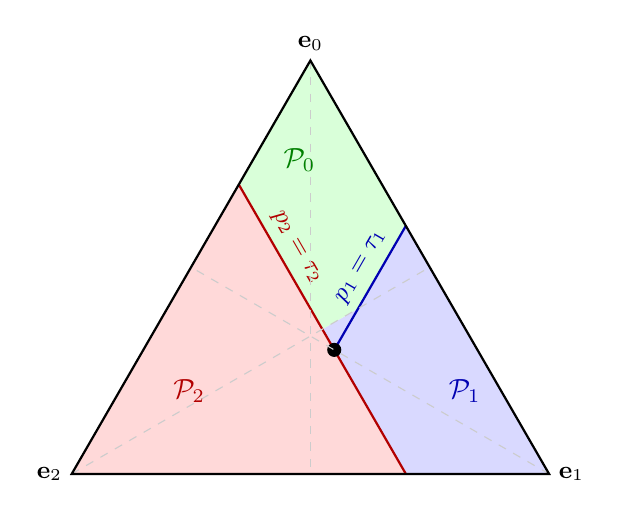
\begin{tikzpicture}[font=\sffamily, scale=0.7]

    % Vertices
    \coordinate (T) at (0, 5);          % Class 0 (p_0=1)
    \coordinate (R) at (4.33, -2.5);    % Class 1 (p_1=1)
    \coordinate (L) at (-4.33, -2.5);   % Class 2 (p_2=1)

    % Threshold contour endpoints:
    % p_2 = 0.30 line:
    %   Top-Left edge (p_1=0): (0.70, 0, 0.30) -> (-1.299, 2.75)
    %   Right-Left edge (p_0=0): (0, 0.70, 0.30) -> (1.732, -2.5)
    \coordinate (T2a) at (-1.299, 2.75);
    \coordinate (T2b) at (1.732, -2.5);

    % p_1 = 0.40 line:
    %   Top-Right edge (p_2=0): (0.60, 0.40, 0) -> (1.732, 2.0)
    %   Right-Left edge (p_0=0): (0, 0.40, 0.60) -> (-0.866, -2.5)
    \coordinate (T1a) at (1.732, 2.0);
    \coordinate (T1b) at (-0.866, -2.5);

    % Intersection of p_2=0.30 and p_1=0.40: (0.30, 0.40, 0.30) -> (0.433, -0.25)
    \coordinate (Corner) at (0.433, -0.25);

    % ===== Region fills =====

    % Argmax median (p_0=p_1) intersects the fallback region at two points:
    %   MedOnBlue: on p_1=0.40 line at (0.35, 0.35, 0.30) -> (0.2165, 0.125)
    %     Wait: (p0=0.35, p1=0.35, p2=0.30) -> x=4.33*(0.35-0.30)=0.2165, y=7.5*0.35-2.5=0.125
    %   MedOnP1: on p_1=0.40 line at (0.30, 0.40, 0.30)... that's Corner itself
    %     Actually: median L-MidTR intersects p_1=0.40 at (0.30, 0.40, 0.30)
    %     but Corner=(0.30, 0.40, 0.30) IS the intersection of p1=0.40 and p2=0.30.
    %     The median hits p_1=0.40 at (p0, 0.40, p2) where p0=p1=0.40... wait no.
    %     p0=p1 and p1=0.40 means p0=0.40, p2=0.20.
    %     -> x=4.33*(0.40-0.20)=0.866, y=7.5*0.40-2.5=0.5
    \coordinate (MedOnRed) at (0.2165, 0.125);  % p0=p1 meets p2=0.30
    \coordinate (MedOnBlue) at (0.866, 0.5);     % p0=p1 meets p1=0.40

    % Class 2 (red, priority 1): p_2 >= 0.30
    \fill[red!15] (T2a) -- (T2b) -- (L) -- cycle;

    % Class 1 (blue, priority 2): p_2 < 0.30 AND p_1 >= 0.40
    \fill[blue!15] (T1a) -- (Corner) -- (T2b) -- (R) -- cycle;

    % Class 1 (blue, fallback argmax): p_2 < 0.30 AND p_1 < 0.40 AND p_1 > p_0
    \fill[blue!15] (MedOnBlue) -- (Corner) -- (MedOnRed) -- cycle;

    % Class 0 (green, fallback argmax): p_2 < 0.30 AND p_1 < 0.40 AND p_0 > p_1
    \fill[green!15] (T) -- (T1a) -- (MedOnBlue) -- (MedOnRed) -- (T2a) -- cycle;

    % ===== Threshold contour lines =====

    % p_2 = tau_2 line (separates class 2 from rest)
    \draw[thick, red!70!black] (T2a) -- (T2b)
        node[sloped, above, pos=0.25, font=\small, red!70!black] {$p_2 = \tau_2$};

    % p_1 = tau_1 line (separates class 1 from class 0, within p_2 < tau_2)
    \draw[thick, blue!70!black] (T1a) -- (Corner)
        node[sloped, above, pos=0.4, font=\small, blue!70!black] {$p_1 = \tau_1$};

    % Corner marker (the "step" — key visual)
    \node[circle, fill=black, inner sep=1.8pt] at (Corner) {};

    % ===== Argmax boundaries (dashed, for comparison) =====
    \coordinate (MidTR) at (2.165, 1.25);
    \coordinate (MidTL) at (-2.165, 1.25);
    \coordinate (MidRL) at (0, -2.5);
    \draw[dashed, gray!40, thin] (L) -- (MidTR);
    \draw[dashed, gray!40, thin] (R) -- (MidTL);
    \draw[dashed, gray!40, thin] (T) -- (MidRL);

    % ===== Triangle frame =====
    \draw[thick] (T) -- (R) -- (L) -- cycle;

    % ===== Labels =====

    % Vertex labels
    \node[above, font=\small] at (T) {$\mathbf{e}_0$};
    \node[right, font=\small] at (R) {$\mathbf{e}_1$};
    \node[left, font=\small] at (L) {$\mathbf{e}_2$};

    % Region labels
    \node[green!50!black, font=\normalsize\bfseries] at (-0.2, 3.2) {$\mathcal{P}_0$};
    \node[blue!70!black, font=\normalsize\bfseries] at (2.8, -1.0) {$\mathcal{P}_1$};
    \node[red!70!black, font=\normalsize\bfseries] at (-2.2, -1.0) {$\mathcal{P}_2$};

\end{tikzpicture}
\end{document}

    \caption{Decision regions induced by sequential selection with priority order $\mathrm{ord} = (2, 1, 0)$ and thresholds $\tau_2 = 0.30$, $\tau_1 = 0.40$ on the 3-class probability simplex. Class~2 is evaluated first: any point with $p_2 \ge \tau_2$ is claimed by class~2 regardless of other probabilities, creating the red region. Class~1 is evaluated next in the complement, and class~0 receives the fallback.}\label{fig:sequential_selection}
\end{figure}

\section{Limitations of parallel-shift partitions}

Every boundary normal of $\mathcal{H}_{PS}$ is locked to $\mathbf{n}_{ij} = \mathbf{c}_i - \mathbf{c}_j$, a fixed expressivity cost: the rule can translate the partition but cannot rotate or curve any boundary. Two regimes make this constraint binding.

\subsection{Error-covariance misalignment}
When the estimator's error has directional structure that is not aligned with the cost-matrix differences, the risk-minimizing boundary in estimate space need not be normal to $\mathbf{n}_{ij} = \mathbf{c}_i - \mathbf{c}_j$. If $\Sigma_\epsilon$ is the covariance of $\boldsymbol{\epsilon}(x) = \hat{\mathbf{p}}(x) - \boldsymbol{\eta}(x)$ and its principal axes are not aligned with $\mathbf{c}_i - \mathbf{c}_j$, the orientation that minimizes risk depends on $\Sigma_\epsilon$ and can differ from the analytical normal. $\mathcal{H}_{PS}$ fixes every boundary normal at $\mathbf{n}_{ij}$, so it cannot represent such a rotation and the mismatch contributes to excess risk that the class has no parameter to remove.

\subsection{Non-linear calibration bias}
When the systematic distortion $\Psi$ of Section~\ref{sec:analytical_fragility} is non-linear (for example the saturation of softmax outputs in deep networks, or the prior shrinkage of in-context predictors), the pre-image $\Psi^{-1}(\mathcal{B}_{ij})$ of the analytical boundary is in general a curved manifold in estimate space rather than a hyperplane. A flat parallel-shift boundary can only approximate it, with an approximation error that grows with the local curvature of $\Psi$ and that $\mathcal{H}_{PS}$ has no parameter to reduce.

Both regimes motivate a hypothesis class whose boundary normals can rotate, which $\mathcal{H}_{PS}$ forbids. The Voronoi partition class of Chapter~\ref{sec:voronoi_tessellation} provides this, with $K(K-1)$ prototype parameters and boundary rotations that $\mathcal{H}_{PS}$ cannot represent.
